\newpage
\section{Экспериментальная часть}

Необходимо протестировать алгоритм перебора и провести исследование.

\subsection{Примеры работы}

На рисунках \ref{img:zero_arg}, \ref{img:not_exist} и \ref{img:good} представлены примеры работы программы.

\begin{figure}[H]
    \centering
    
\includegraphics[scale=0.4]{zero_arg}
    \caption{Запуск без аргументов}
    \label{img:zero_arg}
\end{figure}

\begin{figure}[H]
    \centering
    
\includegraphics[scale=0.4]{not_exist}
    \caption{Запуск с несуществующим файлом}
    \label{img:not_exist}
\end{figure}

\begin{figure}[H]
    \centering
    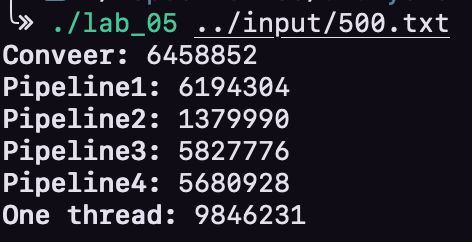
\includegraphics[scale=1]{good}
    \caption{Корректный файл}
    \label{img:good}
\end{figure}

\subsection{Результаты тестирования}

Результаты тестирования представлены на таблице \ref{table:test_result}.

\begin{table}[H]
    \caption{Результаты}
    \label{table:test_result}
    \centering
    \begin{tabular}{|l||c|}
        \hline
        Входной граф & Резуьтат \\
        \hline
        \hline
        \hline
        4 & \\
        0 1 2 3 & \\
        1 0 3 4 & 0 1 2 3 \\
        2 3 0 5 & dist = 12 \\
        3 4 5 0 & \\
        \hline
        5 & \\
        0 1 -1 3 4 & \\
        1 0 3 4 5 & 0 1 3 4 2 \\
        -1 3 0 5 -1 & dist = 10 \\
        3 4 5 0 7 & \\
        4 5 -1 7 0 & \\
        \hline
        5 & \\
        0 5 8 9 2 & \\
        5 0 3 3 4 & 0 2 1 3 4 \\
        8 3 0 7 6 & dist = 17 \\
        9 3 7 0 1 & \\
        2 4 6 1 0 & \\
        \hline
    \end{tabular}
\end{table}

Все тесты пройдены успешно.

\subsection{Выбор коэффициентов}

Проведено исследование сравнения результатов поного перебора с муравьиным алгоритмом с различными
значениями коээфициентов
($0 \le \rho \le 1;\ 0.2 \le \alpha \le 0.8;\ \alpha + \beta = 1;\ 0.2 \le \beta \le 1;\ 10 \le t_{\max} \le 1000$).

$\alpha$ -- коэффициент стадности, $\beta$ -- коэффициент жадности, $t_{\max}$ -- количество итераций времени, $\rho$ -- cкорость
испарения фероменов.

\begin{table}[H]
    \centering
    \caption{5 городов}
    \label{table:city5}
    \begin{tabular}{|c|c|c|c|c|c|}
        \hline
        $\alpha$ & $\beta$ & $\rho$ & $t_{max}$ & Длина маршрута муравья & Длина маршрута перебора \\
        \hline
        0.2 & 0.8 & 0 & 10 & 17 & 17 \\
        0.2 & 0.8 & 0 & 60 & 17 & 17 \\
        0.2 & 0.8 & 0 & 110 & 17 & 17 \\
        0.2 & 0.8 & 0 & 160 & 17 & 17 \\
        ... & ... & ... & ... & ... & ... \\
        0.8 & 0.2 & 1 & 510 & 17 & 17 \\
        0.8 & 0.2 & 1 & 560 & 17 & 17 \\
        0.8 & 0.2 & 1 & 610 & 17 & 17 \\
        0.8 & 0.2 & 1 & 660 & 17 & 17 \\
        \hline
    \end{tabular}
\end{table}

\begin{table}[H]
    \centering
    \caption{8 городов}
    \label{table:city15}
    \begin{tabular}{|c|c|c|c|c|c|}
        \hline
        $\alpha$ & $\beta$ & $\rho$ & $t_{max}$ & Длина маршрута муравья & Длина маршрута перебора \\
        \hline
        0.2 & 0.8 & 0 & 50 & 22 & 22 \\
        0.2 & 0.8 & 0 & 100 & 22 & 22 \\
        0.2 & 0.8 & 0 & 150 & 22 & 22 \\
        0.2 & 0.8 & 0 & 200 & 22 & 22 \\
        0.2 & 0.8 & 0 & 250 & 22 & 22 \\
        0.2 & 0.8 & 0 & 300 & 22 & 22 \\
        0.2 & 0.8 & 0 & 350 & 25 & 22 \\
        0.2 & 0.8 & 0 & 400 & 25 & 22 \\
        0.2 & 0.8 & 0 & 450 & 25 & 22 \\
        0.2 & 0.8 & 0 & 500 & 25 & 22 \\
        0.2 & 0.8 & 0 & 550 & 25 & 22 \\
        0.2 & 0.8 & 0 & 600 & 25 & 22 \\
        0.2 & 0.8 & 0 & 650 & 23 & 22 \\
        ... & ... & ... & ... & ... & ... \\
        0.4 & 0.6 & 0 & 1200 & 22 & 22 \\
        0.4 & 0.6 & 0.25 & 50 & 28 & 22 \\
        0.4 & 0.6 & 0.25 & 100 & 28 & 22 \\
        0.4 & 0.6 & 0.25 & 150 & 28 & 22 \\
        0.4 & 0.6 & 0.25 & 200 & 28 & 22 \\
        0.4 & 0.6 & 0.25 & 250 & 28 & 22 \\
        0.4 & 0.6 & 0.25 & 300 & 23 & 22 \\
        0.4 & 0.6 & 0.25 & 350 & 23 & 22 \\
        0.4 & 0.6 & 0.25 & 400 & 23 & 22 \\
        0.4 & 0.6 & 0.25 & 450 & 23 & 22 \\
        0.4 & 0.6 & 0.25 & 500 & 23 & 22 \\
        0.4 & 0.6 & 0.25 & 550 & 23 & 22 \\
        0.4 & 0.6 & 0.25 & 600 & 22 & 22 \\
        ... & ... & ... & ... & ... & ... \\
        0.4 & 0.6 & 0.5 & 1200 & 22 & 22 \\
        0.4 & 0.6 & 0.75 & 50 & 31 & 22 \\
        0.4 & 0.6 & 0.75 & 100 & 23 & 22 \\
        ... & ... & ... & ... & ... & ... \\
        0.8 & 0.2 & 1 & 1150 & 22 & 22 \\
        0.8 & 0.2 & 1 & 1200 & 22 & 22 \\
        \hline
    \end{tabular}
\end{table}

\begin{table}[H]
    \centering
    \caption{10 городов}
    \label{table:city10}
    \begin{tabular}{|c|c|c|c|c|c|}
        \hline
        $\alpha$ & $\beta$ & $\rho$ & $t_{max}$ & Длина маршрута муравья & Длина маршрута перебора \\
        \hline
        0.2 & 0.8 & 0 & 50 & 31 & 16 \\
        0.2 & 0.8 & 0 & 100 & 31 & 16 \\
        0.2 & 0.8 & 0 & 150 & 31 & 16 \\
        0.2 & 0.8 & 0 & 200 & 31 & 16 \\
        0.2 & 0.8 & 0 & 250 & 31 & 16 \\
        0.2 & 0.8 & 0 & 300 & 25 & 16 \\
        0.2 & 0.8 & 0 & 350 & 25 & 16 \\
        0.2 & 0.8 & 0 & 400 & 25 & 16 \\
        0.2 & 0.8 & 0 & 450 & 25 & 16 \\
        0.2 & 0.8 & 0 & 500 & 25 & 16 \\
        0.2 & 0.8 & 0 & 550 & 25 & 16 \\
        0.2 & 0.8 & 0 & 600 & 25 & 16 \\
        0.2 & 0.8 & 0 & 650 & 31 & 16 \\
        0.2 & 0.8 & 0 & 700 & 31 & 16 \\
        0.2 & 0.8 & 0 & 750 & 31 & 16 \\
        ... & ... & ... & ... & ... & ... \\
        0.4 & 0.6 & 0.75 & 1100 & 25 & 16 \\
        0.4 & 0.6 & 0.75 & 1150 & 16 & 16 \\
        0.4 & 0.6 & 0.75 & 1200 & 16 & 16 \\
        0.4 & 0.6 & 1 & 50 & 33 & 16 \\
        ... & ... & ... & ... & ... & ...\\
        0.8 & 0.2 & 1 & 850 & 26 & 16 \\
        0.8 & 0.2 & 1 & 900 & 16 & 16 \\
        0.8 & 0.2 & 1 & 950 & 16 & 16 \\
        0.8 & 0.2 & 1 & 1000 & 16 & 16 \\
        0.8 & 0.2 & 1 & 1050 & 30 & 16 \\
        0.8 & 0.2 & 1 & 1100 & 30 & 16 \\
        0.8 & 0.2 & 1 & 1150 & 30 & 16 \\
        0.8 & 0.2 & 1 & 1200 & 24 & 16 \\
        \hline
    \end{tabular}
\end{table}

\subsection{Выводы}

Из исследования можно сделать вывод, что для 8 городов и больше
лучше всего подходит соотношение $\alpha = 0.4$ и $\beta = 0.6$,
приходится использовать $t_{\min} \geq 1000$ чтобы алгоритм работал
максимально точно. А значение $\rho$ можно
использовать в промежутке $[0 ; 0.75]$.
